% 例 2：▱ABCD, 对角线交于 O, E 在 OA 上, F 在 OC 上, OE = OF
\documentclass[tikz,border=4pt]{standalone}
\usepackage{ctex}
\usepackage{amsmath}
\usetikzlibrary{calc, decorations.markings}
\begin{document}
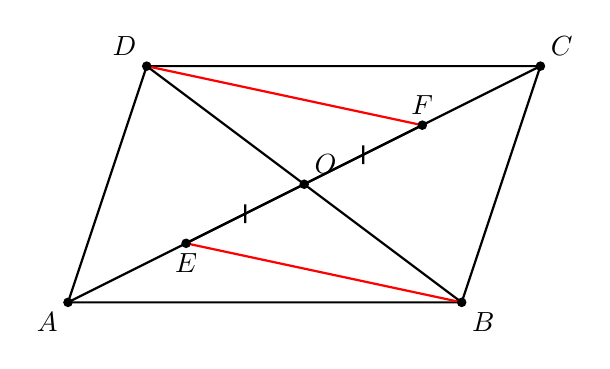
\begin{tikzpicture}[scale=1.0, thick,
  tickone/.style={postaction={decorate, decoration={markings,
    mark=at position 0.5 with {\draw (-1.5pt,-3pt) -- (1.5pt,3pt);}}}},
]
  \coordinate (A) at (0,0);
  \coordinate (B) at (5,0);
  \coordinate (C) at (6,3);
  \coordinate (D) at (1,3);
  \coordinate (O) at ($(A)!0.5!(C)$);
  \coordinate (E) at ($(O)!0.5!(A)$);
  \coordinate (F) at ($(O)!0.5!(C)$);
  \draw (A) -- (B) -- (C) -- (D) -- cycle;
  \draw (A) -- (C);
  \draw (B) -- (D);
  \draw[red, thick] (B) -- (E);
  \draw[red, thick] (D) -- (F);
  % OE 与 OF 等长标记
  \draw[tickone] (O) -- (E);
  \draw[tickone] (O) -- (F);
  \foreach \pt in {A,B,C,D,O,E,F} \filldraw (\pt) circle (1.3pt);
  \node[below left]  at (A) {$A$};
  \node[below right] at (B) {$B$};
  \node[above right] at (C) {$C$};
  \node[above left]  at (D) {$D$};
  \node[above right] at (O) {$O$};
  \node[below]       at (E) {$E$};
  \node[above]       at (F) {$F$};
\end{tikzpicture}
\end{document}
